% tikz_eps0.tex -- the explicit constant epsilon_0 of Theorem 2.18 (Section 7.13).
%   (a) The chain of explicit bounds from twenty-four directions with inner products at most
%       1/2 + kappa to the volume bound, with the number each step produces
%       (multi_cap/explicit_eps0.py and its log).
%   (b) To scale, on logarithmic axes: the lower bound q_min f(u) of sigma_2 near its double zero
%       u = 0, with f(u) = (u+1)(u+1/2)^2 u^2 (1/2 - u) and q_min = 2.62e-4, against the level
%       E(24, kappa) = 2.35e-12 that the sign-changing sum-of-squares terms can reach; the bound
%       clears the level at |u| = delta = 3e-4 (2.94e-12 there), so every inner product lies within
%       delta of a zero.  The other double zero, -1/2, gives the same picture.
% Build:  pdflatex tikz_eps0.tex && pdftoppm -r 500 -png -singlefile tikz_eps0.pdf ../figures/fig_tikz_eps0
\documentclass[border=4pt]{standalone}
\usepackage{tikz}
\usepackage{pgfplots}
\pgfplotsset{compat=1.17}
\usetikzlibrary{positioning,arrows.meta,calc}
\usepackage[T1]{fontenc}
\usepackage{lmodern}
\usepackage{amsmath,amssymb}
\definecolor{cblue}{HTML}{2A78D6}
\definecolor{corange}{HTML}{EB6834}
\definecolor{caqua}{HTML}{1BAF7A}
\definecolor{cviolet}{HTML}{4A3AA7}
\definecolor{cink}{HTML}{0B0B0B}
\definecolor{cink2}{HTML}{52514E}
\definecolor{cink3}{HTML}{8B8A85}
\begin{document}
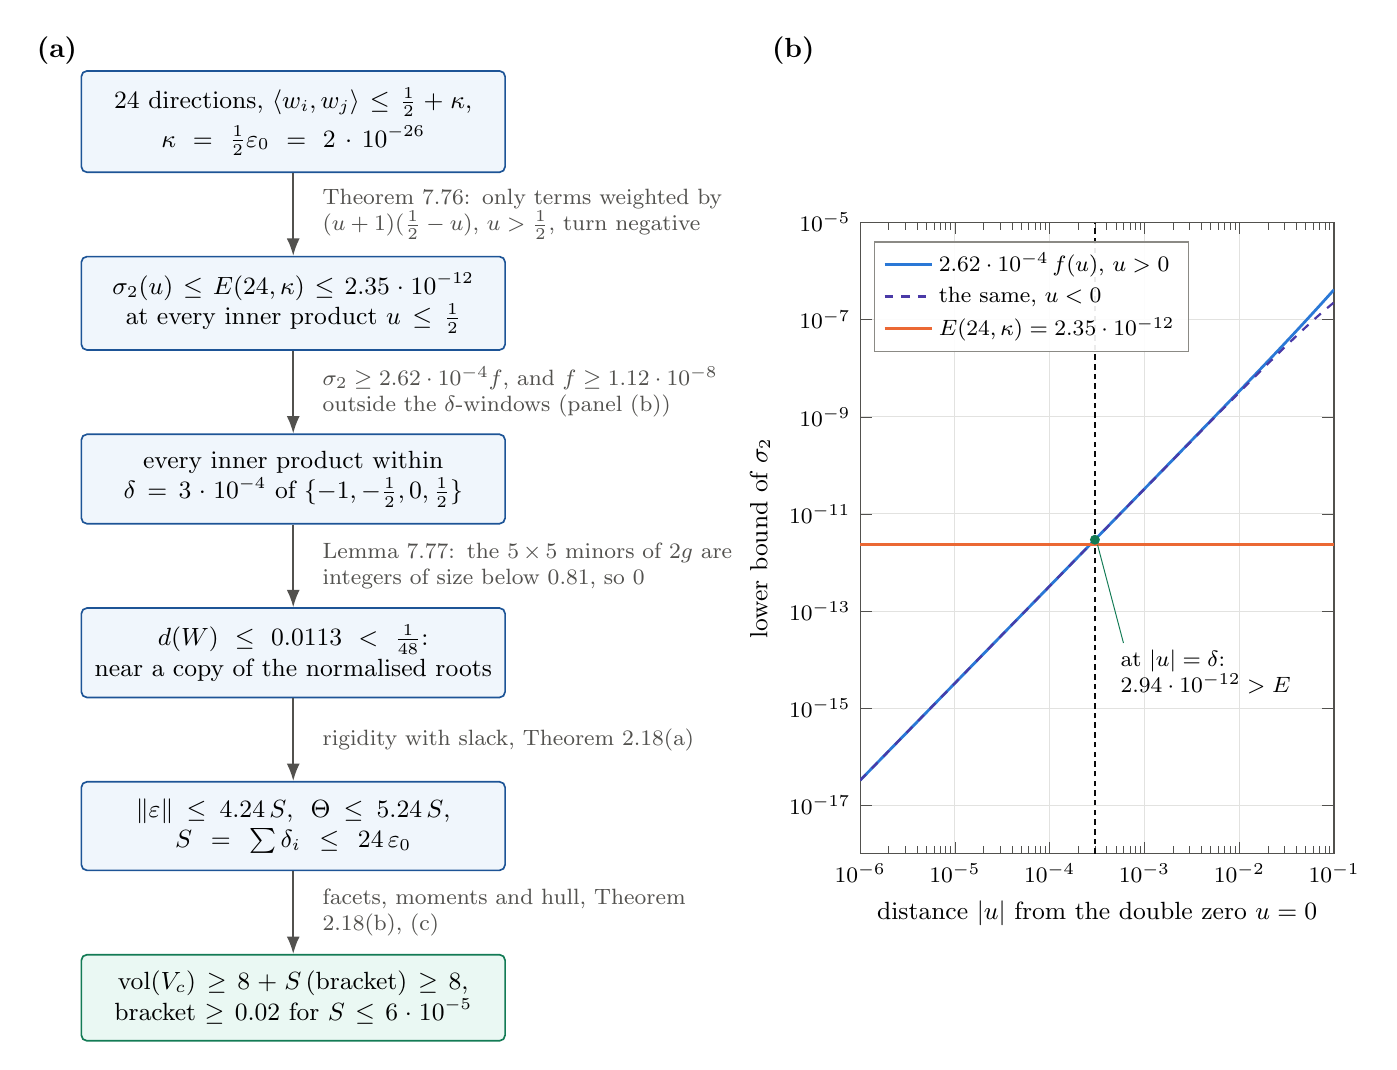
\begin{tikzpicture}[font=\small,
  state/.style={draw=cblue!70!black, fill=cblue!7, rounded corners=2pt, line width=0.6pt,
                align=center, text width=5.1cm, inner xsep=4pt, inner ysep=6pt, minimum height=1.05cm},
  stepnote/.style={font=\footnotesize, text=cink2, align=left, text width=5.2cm, anchor=west},
  arr/.style={-{Latex[length=2.2mm]}, line width=0.6pt, cink2}]
%% ------------------------------------------------------------------ (a)
\node[font=\bfseries] at (-3.0,0.9) {(a)};
\node[state] (s1) at (0,0) {$24$ directions, $\langle w_i,w_j\rangle\le\tfrac12+\kappa$,\\[3pt] $\kappa=\tfrac12\varepsilon_0=2\cdot10^{-26}$};
\node[state] (s2) [below=1.05cm of s1] {$\sigma_2(u)\le E(24,\kappa)\le2.35\cdot10^{-12}$\\ at every inner product $u\le\tfrac12$};
\node[state] (s3) [below=1.05cm of s2] {every inner product within\\ $\delta=3\cdot10^{-4}$ of $\{-1,-\tfrac12,0,\tfrac12\}$};
\node[state] (s4) [below=1.05cm of s3] {$d(W)\le0.0113<\tfrac1{48}$:\\ near a copy of the normalised roots};
\node[state] (s5) [below=1.05cm of s4] {$\|\varepsilon\|\le4.24\,S$, $\ \Theta\le5.24\,S$,\\ $S=\sum\delta_i\le24\,\varepsilon_0$};
\node[state, draw=caqua!70!black, fill=caqua!9] (s6) [below=1.05cm of s5] {$\operatorname{vol}(V_c)\ge8+S\,(\text{bracket})\ge8$,\\ bracket $\ge0.02$ for $S\le6\cdot10^{-5}$};
\foreach \a/\b in {s1/s2,s2/s3,s3/s4,s4/s5,s5/s6} \draw[arr] (\a.south) -- (\b.north);
\node[stepnote] at ($(s1.south)!0.5!(s2.north)+(0.25,0)$) {Theorem 7.76: only terms weighted by\\ $(u+1)(\tfrac12-u)$, $u>\tfrac12$, turn negative};
\node[stepnote] at ($(s2.south)!0.5!(s3.north)+(0.25,0)$) {$\sigma_2\ge2.62\cdot10^{-4}f$, and $f\ge1.12\cdot10^{-8}$\\ outside the $\delta$-windows (panel (b))};
\node[stepnote] at ($(s3.south)!0.5!(s4.north)+(0.25,0)$) {Lemma 7.77: the $5\times5$ minors of $2g$ are\\ integers of size below $0.81$, so $0$};
\node[stepnote] at ($(s4.south)!0.5!(s5.north)+(0.25,0)$) {rigidity with slack, Theorem 2.18(a)};
\node[stepnote] at ($(s5.south)!0.5!(s6.north)+(0.25,0)$) {facets, moments and hull, Theorem 2.18(b), (c)};
%% ------------------------------------------------------------------ (b)
\node[font=\bfseries] at (6.35,0.9) {(b)};
\begin{axis}[at={(7.2cm,-9.3cm)}, anchor=south west, width=7.6cm, height=9.6cm,
  xmode=log, ymode=log, xmin=1e-6, xmax=1e-1, ymin=1e-18, ymax=1e-5,
  xlabel={distance $|u|$ from the double zero $u=0$}, ylabel={lower bound of $\sigma_2$},
  label style={font=\small}, tick label style={font=\footnotesize},
  axis line style={cink2}, tick style={cink2}, grid=major, grid style={cink3!25},
  legend cell align=left, legend style={font=\footnotesize, at={(0.03,0.97)}, anchor=north west, draw=cink3, fill=white, fill opacity=0.92, text opacity=1}]
\addplot[domain=1e-6:1e-1, samples=160, line width=1.0pt, cblue]
  {2.62e-4*(1+x)*(0.5+x)^2*x^2*(0.5-x)};
\addlegendentry{$2.62\cdot10^{-4}\,f(u)$, $u>0$}
\addplot[domain=1e-6:1e-1, samples=160, line width=0.8pt, cviolet, dashed]
  {2.62e-4*(1-x)*(0.5-x)^2*x^2*(0.5+x)};
\addlegendentry{the same, $u<0$}
\addplot[domain=1e-6:1e-1, samples=2, line width=0.9pt, corange] {2.35e-12};
\addlegendentry{$E(24,\kappa)=2.35\cdot10^{-12}$}
\draw[cink, line width=0.6pt, dash pattern=on 2pt off 1.5pt] (axis cs:3e-4,1e-18) -- (axis cs:3e-4,1e-5);
\fill[caqua!70!black] (axis cs:3e-4,2.94e-12) circle (1.8pt);
\node[font=\footnotesize, anchor=north west, align=left, inner sep=1.5pt]
  at (axis cs:5e-4,2e-14) {at $|u|=\delta$:\\ $2.94\cdot10^{-12}>E$};
\draw[caqua!70!black, line width=0.35pt] (axis cs:6e-4,2.2e-14) -- (axis cs:3.2e-4,2.3e-12);
\end{axis}
\end{tikzpicture}
\end{document}
